% Options for packages loaded elsewhere
\PassOptionsToPackage{unicode}{hyperref}
\PassOptionsToPackage{hyphens}{url}
\PassOptionsToPackage{dvipsnames,svgnames,x11names}{xcolor}
%
\documentclass[
  a4paper,
]{report}

\usepackage{amsmath,amssymb}
\usepackage{setspace}
\usepackage{iftex}
\ifPDFTeX
  \usepackage[T1]{fontenc}
  \usepackage[utf8]{inputenc}
  \usepackage{textcomp} % provide euro and other symbols
\else % if luatex or xetex
  \usepackage{unicode-math}
  \defaultfontfeatures{Scale=MatchLowercase}
  \defaultfontfeatures[\rmfamily]{Ligatures=TeX,Scale=1}
\fi
\usepackage{lmodern}
\ifPDFTeX\else  
    % xetex/luatex font selection
\fi
% Use upquote if available, for straight quotes in verbatim environments
\IfFileExists{upquote.sty}{\usepackage{upquote}}{}
\IfFileExists{microtype.sty}{% use microtype if available
  \usepackage[]{microtype}
  \UseMicrotypeSet[protrusion]{basicmath} % disable protrusion for tt fonts
}{}
\usepackage{xcolor}
\usepackage[left=3cm,textwidth=12cm,marginparsep=0.5cm,marginparwidth=4.5cm]{geometry}
\setlength{\emergencystretch}{3em} % prevent overfull lines
\setcounter{secnumdepth}{5}
% Make \paragraph and \subparagraph free-standing
\makeatletter
\ifx\paragraph\undefined\else
  \let\oldparagraph\paragraph
  \renewcommand{\paragraph}{
    \@ifstar
      \xxxParagraphStar
      \xxxParagraphNoStar
  }
  \newcommand{\xxxParagraphStar}[1]{\oldparagraph*{#1}\mbox{}}
  \newcommand{\xxxParagraphNoStar}[1]{\oldparagraph{#1}\mbox{}}
\fi
\ifx\subparagraph\undefined\else
  \let\oldsubparagraph\subparagraph
  \renewcommand{\subparagraph}{
    \@ifstar
      \xxxSubParagraphStar
      \xxxSubParagraphNoStar
  }
  \newcommand{\xxxSubParagraphStar}[1]{\oldsubparagraph*{#1}\mbox{}}
  \newcommand{\xxxSubParagraphNoStar}[1]{\oldsubparagraph{#1}\mbox{}}
\fi
\makeatother


\providecommand{\tightlist}{%
  \setlength{\itemsep}{0pt}\setlength{\parskip}{0pt}}\usepackage{longtable,booktabs,array}
\usepackage{calc} % for calculating minipage widths
% Correct order of tables after \paragraph or \subparagraph
\usepackage{etoolbox}
\makeatletter
\patchcmd\longtable{\par}{\if@noskipsec\mbox{}\fi\par}{}{}
\makeatother
% Allow footnotes in longtable head/foot
\IfFileExists{footnotehyper.sty}{\usepackage{footnotehyper}}{\usepackage{footnote}}
\makesavenoteenv{longtable}
\usepackage{graphicx}
\makeatletter
\def\maxwidth{\ifdim\Gin@nat@width>\linewidth\linewidth\else\Gin@nat@width\fi}
\def\maxheight{\ifdim\Gin@nat@height>\textheight\textheight\else\Gin@nat@height\fi}
\makeatother
% Scale images if necessary, so that they will not overflow the page
% margins by default, and it is still possible to overwrite the defaults
% using explicit options in \includegraphics[width, height, ...]{}
\setkeys{Gin}{width=\maxwidth,height=\maxheight,keepaspectratio}
% Set default figure placement to htbp
\makeatletter
\def\fps@figure{htbp}
\makeatother

\usepackage{amsmath}
\usepackage{amsthm}
\usepackage{amssymb}
\usepackage{stmaryrd}
\usepackage{mathpartir}
\usepackage{cancel}

\usepackage{booktabs}

%\usepackage{unicode-math}
%\setmathfont{STIXTwoMath-Regular.otf}


\usepackage{fontawesome5}

\usepackage{fontspec,unicode-math}
\usepackage{newunicodechar}

\newunicodechar{👁}{\text{\faIcon[regular]{eye}}}

%\input{style/macros.md}
\makeatletter
\@ifpackageloaded{tcolorbox}{}{\usepackage[skins,breakable]{tcolorbox}}
\@ifpackageloaded{fontawesome5}{}{\usepackage{fontawesome5}}
\definecolor{quarto-callout-color}{HTML}{909090}
\definecolor{quarto-callout-note-color}{HTML}{0758E5}
\definecolor{quarto-callout-important-color}{HTML}{CC1914}
\definecolor{quarto-callout-warning-color}{HTML}{EB9113}
\definecolor{quarto-callout-tip-color}{HTML}{00A047}
\definecolor{quarto-callout-caution-color}{HTML}{FC5300}
\definecolor{quarto-callout-color-frame}{HTML}{acacac}
\definecolor{quarto-callout-note-color-frame}{HTML}{4582ec}
\definecolor{quarto-callout-important-color-frame}{HTML}{d9534f}
\definecolor{quarto-callout-warning-color-frame}{HTML}{f0ad4e}
\definecolor{quarto-callout-tip-color-frame}{HTML}{02b875}
\definecolor{quarto-callout-caution-color-frame}{HTML}{fd7e14}
\makeatother
\makeatletter
\@ifpackageloaded{bookmark}{}{\usepackage{bookmark}}
\makeatother
\makeatletter
\@ifpackageloaded{caption}{}{\usepackage{caption}}
\AtBeginDocument{%
\ifdefined\contentsname
  \renewcommand*\contentsname{Table of contents}
\else
  \newcommand\contentsname{Table of contents}
\fi
\ifdefined\listfigurename
  \renewcommand*\listfigurename{List of Figures}
\else
  \newcommand\listfigurename{List of Figures}
\fi
\ifdefined\listtablename
  \renewcommand*\listtablename{List of Tables}
\else
  \newcommand\listtablename{List of Tables}
\fi
\ifdefined\figurename
  \renewcommand*\figurename{Figure}
\else
  \newcommand\figurename{Figure}
\fi
\ifdefined\tablename
  \renewcommand*\tablename{Table}
\else
  \newcommand\tablename{Table}
\fi
}
\@ifpackageloaded{float}{}{\usepackage{float}}
\floatstyle{ruled}
\@ifundefined{c@chapter}{\newfloat{codelisting}{h}{lop}}{\newfloat{codelisting}{h}{lop}[chapter]}
\floatname{codelisting}{Listing}
\newcommand*\listoflistings{\listof{codelisting}{List of Listings}}
\usepackage{amsthm}
\theoremstyle{plain}
\newtheorem{proposition}{Proposition}[section]
\theoremstyle{plain}
\newtheorem{corollary}{Corollary}[section]
\theoremstyle{definition}
\newtheorem{definition}{Definition}[section]
\theoremstyle{plain}
\newtheorem{lemma}{Lemma}[section]
\theoremstyle{definition}
\newtheorem{example}{Example}[section]
\theoremstyle{remark}
\AtBeginDocument{\renewcommand*{\proofname}{Proof}}
\newtheorem*{remark}{Remark}
\newtheorem*{solution}{Solution}
\newtheorem{refremark}{Remark}[section]
\newtheorem{refsolution}{Solution}[section]
\makeatother
\makeatletter
\makeatother
\makeatletter
\@ifpackageloaded{caption}{}{\usepackage{caption}}
\@ifpackageloaded{subcaption}{}{\usepackage{subcaption}}
\makeatother
\makeatletter
\@ifpackageloaded{sidenotes}{}{\usepackage{sidenotes}}
\@ifpackageloaded{marginnote}{}{\usepackage{marginnote}}
\makeatother

\ifLuaTeX
  \usepackage{selnolig}  % disable illegal ligatures
\fi
\usepackage[]{natbib}
\bibliographystyle{plainnat}
\usepackage{bookmark}

\IfFileExists{xurl.sty}{\usepackage{xurl}}{} % add URL line breaks if available
\urlstyle{same} % disable monospaced font for URLs
\hypersetup{
  pdftitle={Generalized Equivalence Checking of Concurrent Programs},
  pdfauthor={Benjamin Bisping},
  colorlinks=true,
  linkcolor={blue},
  filecolor={Maroon},
  citecolor={Blue},
  urlcolor={Blue},
  pdfcreator={LaTeX via pandoc}}


\title{Generalized Equivalence Checking of Concurrent Programs}
\author{Benjamin Bisping}
\date{}

\begin{document}
\maketitle
\begin{abstract}
\ldots{}
\end{abstract}

\renewcommand{\bibsection}{}

\renewcommand*\contentsname{Table of contents}
{
\hypersetup{linkcolor=}
\setcounter{tocdepth}{2}
\tableofcontents
}

\setstretch{1.15}
\bookmarksetup{startatroot}

\chapter*{Welcome}\label{welcome}

\markboth{Welcome}{Welcome}

\begin{tcolorbox}[enhanced jigsaw, breakable, toprule=.15mm, toptitle=1mm, titlerule=0mm, colframe=quarto-callout-warning-color-frame, colbacktitle=quarto-callout-warning-color!10!white, left=2mm, rightrule=.15mm, colback=white, title=\textcolor{quarto-callout-warning-color}{\faExclamationTriangle}\hspace{0.5em}{Warning}, bottomrule=.15mm, opacitybacktitle=0.6, arc=.35mm, coltitle=black, leftrule=.75mm, bottomtitle=1mm, opacityback=0]

This is a work-in-progress document. Handle with care!

\end{tcolorbox}

Purpose: Take the time to explain and present the results of papers X
and Y in a more detailed fashion.

\bookmarksetup{startatroot}

\chapter{Introduction: What's the
difference?}\label{introduction-whats-the-difference}

A long time ago, when working as a student research assistant, I was
tasked with implementing a translation from the process algebra Timed
CSP to Timed Automata. The aim was to bridge between the tools FDR2 and
UPPAAL for Thomas Göthel's dissertation
\citeyearpar{goethel12mechanicalVerificationRTS}. The previous works I
was to base the translations on had serious flaws: One introduced
spurious deadlocks to the model, the other was unable to handle nesting
of choices and parallel composition. Clearly, we had to change the
encoding!

\begin{marginfigure}

\centering{

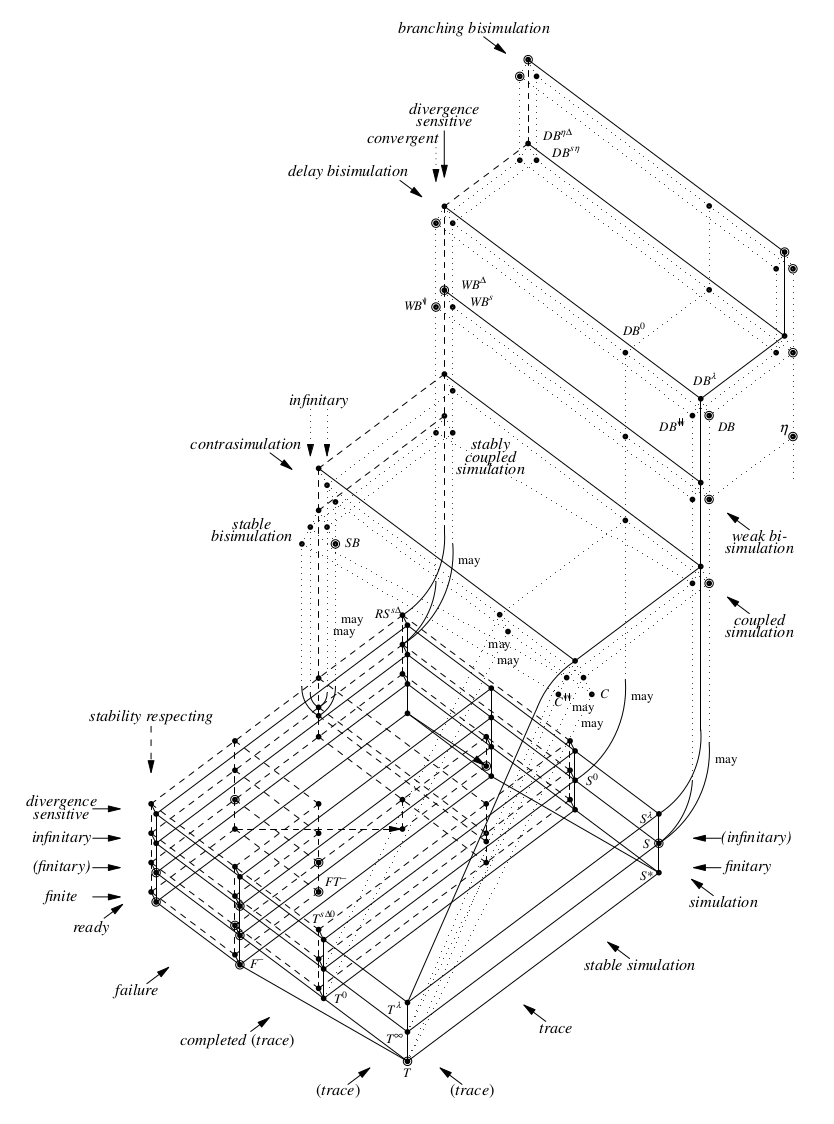
\includegraphics{img/ltbts2.png}

}

\caption{\label{fig-ltbts2-paper}The linear-time--branching-time
spectrum with silent moves as depicted in \citet{glabbeek1993ltbt}.}

\end{marginfigure}%

\ldots{} But how to tell whether our adapted translation would properly
honor the semantics of CSP and Timed Automata? Did we translate CSP
terms to automata \emph{with the same meaning}? This leads to the
question of what counts as \emph{same meaning} in operational semantics.
I took my very first look into an ominous paper on the landscape of
process equivalences, the ``Linear-time--branching-time spectrum II'' by
Rob van Glabbeek \citeyearpar{glabbeek1993ltbt}. The central figure,
reproduced in Figure~\ref{fig-ltbts2-paper}, mesmerized me. How could be
so many different notions of equivalence!

The paper did not really help me back then: I could not wrap my head
around the host of equivalences. But the fascination remained. This
thesis is about an idea how future researchers can tap into the wisdom
of the linear-time--branching-time spectrum and quickly learn what
equivalences relate their models.

\begin{center}\rule{0.5\linewidth}{0.5pt}\end{center}

Can you subtract two programs? Or even more generally: Can you subtract
a specification from a program to see what unspecified behavior remains?
(For your program to be correct, there should be no relevant
difference!)

There is a rich body of work on \emph{process equivalence checking} and
\emph{refinement checking} for programs and specifications. This thesis
argues that most of it can be viewed through one unified lense of
\emph{finding differences} in behavior.

\section{Linear-Time--Branching-Time
Spectroscopy}\label{linear-timebranching-time-spectroscopy}

\section{This Thesis}\label{this-thesis}

\section{Artifacts and Papers}\label{artifacts-and-papers}

\bookmarksetup{startatroot}

\chapter{Preliminaries: Communicating Systems and
Games}\label{preliminaries-communicating-systems-and-games}

\providecommand{\lc}[1]{}

\providecommand{\inverse}[1]{#1^{-1}}
\providecommand{\setminus}{\mathbin{\backslash}}
\providecommand{\powerset}[1]{2^{#1}}
\providecommand{\defiff}{\mathrel{:\!\iff}}
\providecommand{\set}[1]{\{#1\}}
\providecommand{\emptyword}{\texttt{()}}
\providecommand{\identity}[1]{\mathrm{id}_{#1}}

\providecommand{\step}[1]{\xrightarrow{#1}}
\providecommand{\states}{\mathcal{P}}
\providecommand{\system}{\mathcal{S}}
\providecommand{\labels}{\mathcal{L}}
\providecommand{\actions}{\Sigma}
\providecommand{\traces}[1]{\mathsf{Traces}(#1)}

\providecommand{\literal}[1]{\mathsf{#1}}

\providecommand{\grammardef}{\;⩴\;}
\providecommand{\grammaror}{\;\mid\;}

\providecommand{\ccs}{\textsf{CCS}}
\providecommand{\ccschannels}{\mathcal{A}}
\providecommand{\ccsactions}{\actions_\ccs}
\providecommand{\ccslabels}{\labels_\ccs}
\providecommand{\coaction}[1]{\overline{#1}}
\providecommand{\ccsnames}{\mathcal X}
\providecommand{\ccsasg}{\mathcal V}
\providecommand{\ccsprefix}[1]{#1\ldotp\!}
\providecommand{\ccsnull}{\mathbf{0}}
\providecommand{\ccschoice}{+}
\providecommand{\ccspar}{\mid}
\providecommand{\ccsrestrict}{\setminus}

\providecommand{\hml}{\textsf{HML}}
\providecommand{\hmlobs}[1]{\langle #1 \rangle}
\providecommand{\hmland}[2]{\textstyle\bigwedge_{#1 \in #2}}
\providecommand{\hmlands}[1]{\textstyle\bigwedge #1}
\providecommand{\hmltrue}{\top}
\providecommand{\hmlneg}{\neg}

\providecommand{\semantics}[1]{\llbracket #1 \rrbracket}
\providecommand{\semanticsObs}[1]{\semantics{#1}^👁}
\providecommand{\difference}[2]{\Delta(#1,#2)}

\providecommand{\rel}[1]{\mathcal{#1}}

\providecommand{\bpreord}[1]{\preceq_\mathrm{#1}}
\providecommand{\nbpreord}[1]{\not\preceq_\mathrm{#1}}
\providecommand{\bpreordvar}[1]{\preceq_{#1}}
\providecommand{\beq}[1]{\sim_\mathrm{#1}}
\providecommand{\nbeq}[1]{\nsim_\mathrm{#1}}
\providecommand{\beqvar}[1]{\sim_{#1}}
\providecommand{\notions}{\mathbf{N}}
\providecommand{\observations}[1]{\mathcal{O}_\mathrm{#1}}
\providecommand{\observationsvar}[1]{\mathcal{O}_{#1}}

\providecommand{\gamemove}[1]{\mathrel{\smash{›\!\!\frac{#1}{}\!\!›}}}
\providecommand{\gamemoveblank}{\gamemove{\quad}}
\providecommand{\ngamemove}[1]{\mathrel{\smash{{›/\!\!\!\!\frac{#1}{\;}\!\!›}}}}
\providecommand{\ngamemoveblank}{\ngamemove{\quad}}
\providecommand{\game}{\mathcal{G}}
\providecommand{\attackerpos}[1]{{(#1)}_\mathtt{a}}
\providecommand{\defenderpos}[1]{{(#1)}_\mathtt{d}}
\providecommand{\attacker}{{\mathrm{a}}}
\providecommand{\defender}{{\mathrm{d}}}

TODO: Preliminaries\ldots.

\section{Behavior of Programs}\label{behavior-of-programs}

\subsection{Labeled Transition
Systems}\label{labeled-transition-systems}

\begin{definition}[Transition
Systems]\protect\hypertarget{def-ts}{}\label{def-ts}

A \emph{labeled transition system} (LTS)
\(\mathcal{S}=(\mathcal{P},\Sigma,\xrightarrow{})\) consists of

\begin{itemize}
\tightlist
\item
  \(\mathcal{P}\), a set of \emph{states,}
\item
  \(\Sigma\), a set of \emph{actions,} and
\item
  \({\xrightarrow{}} ⊆ \mathcal{P}× \Sigma× \mathcal{P}\), a
  \emph{transition relation}.
\end{itemize}

\end{definition}

\noindent  There is a canonical example used to discuss equivalences
within transition systems. We will take the formulation that Henzinger
used at CAV'23 as seen in Figure~\ref{fig-henzinger}.

\begin{marginfigure}

\centering{

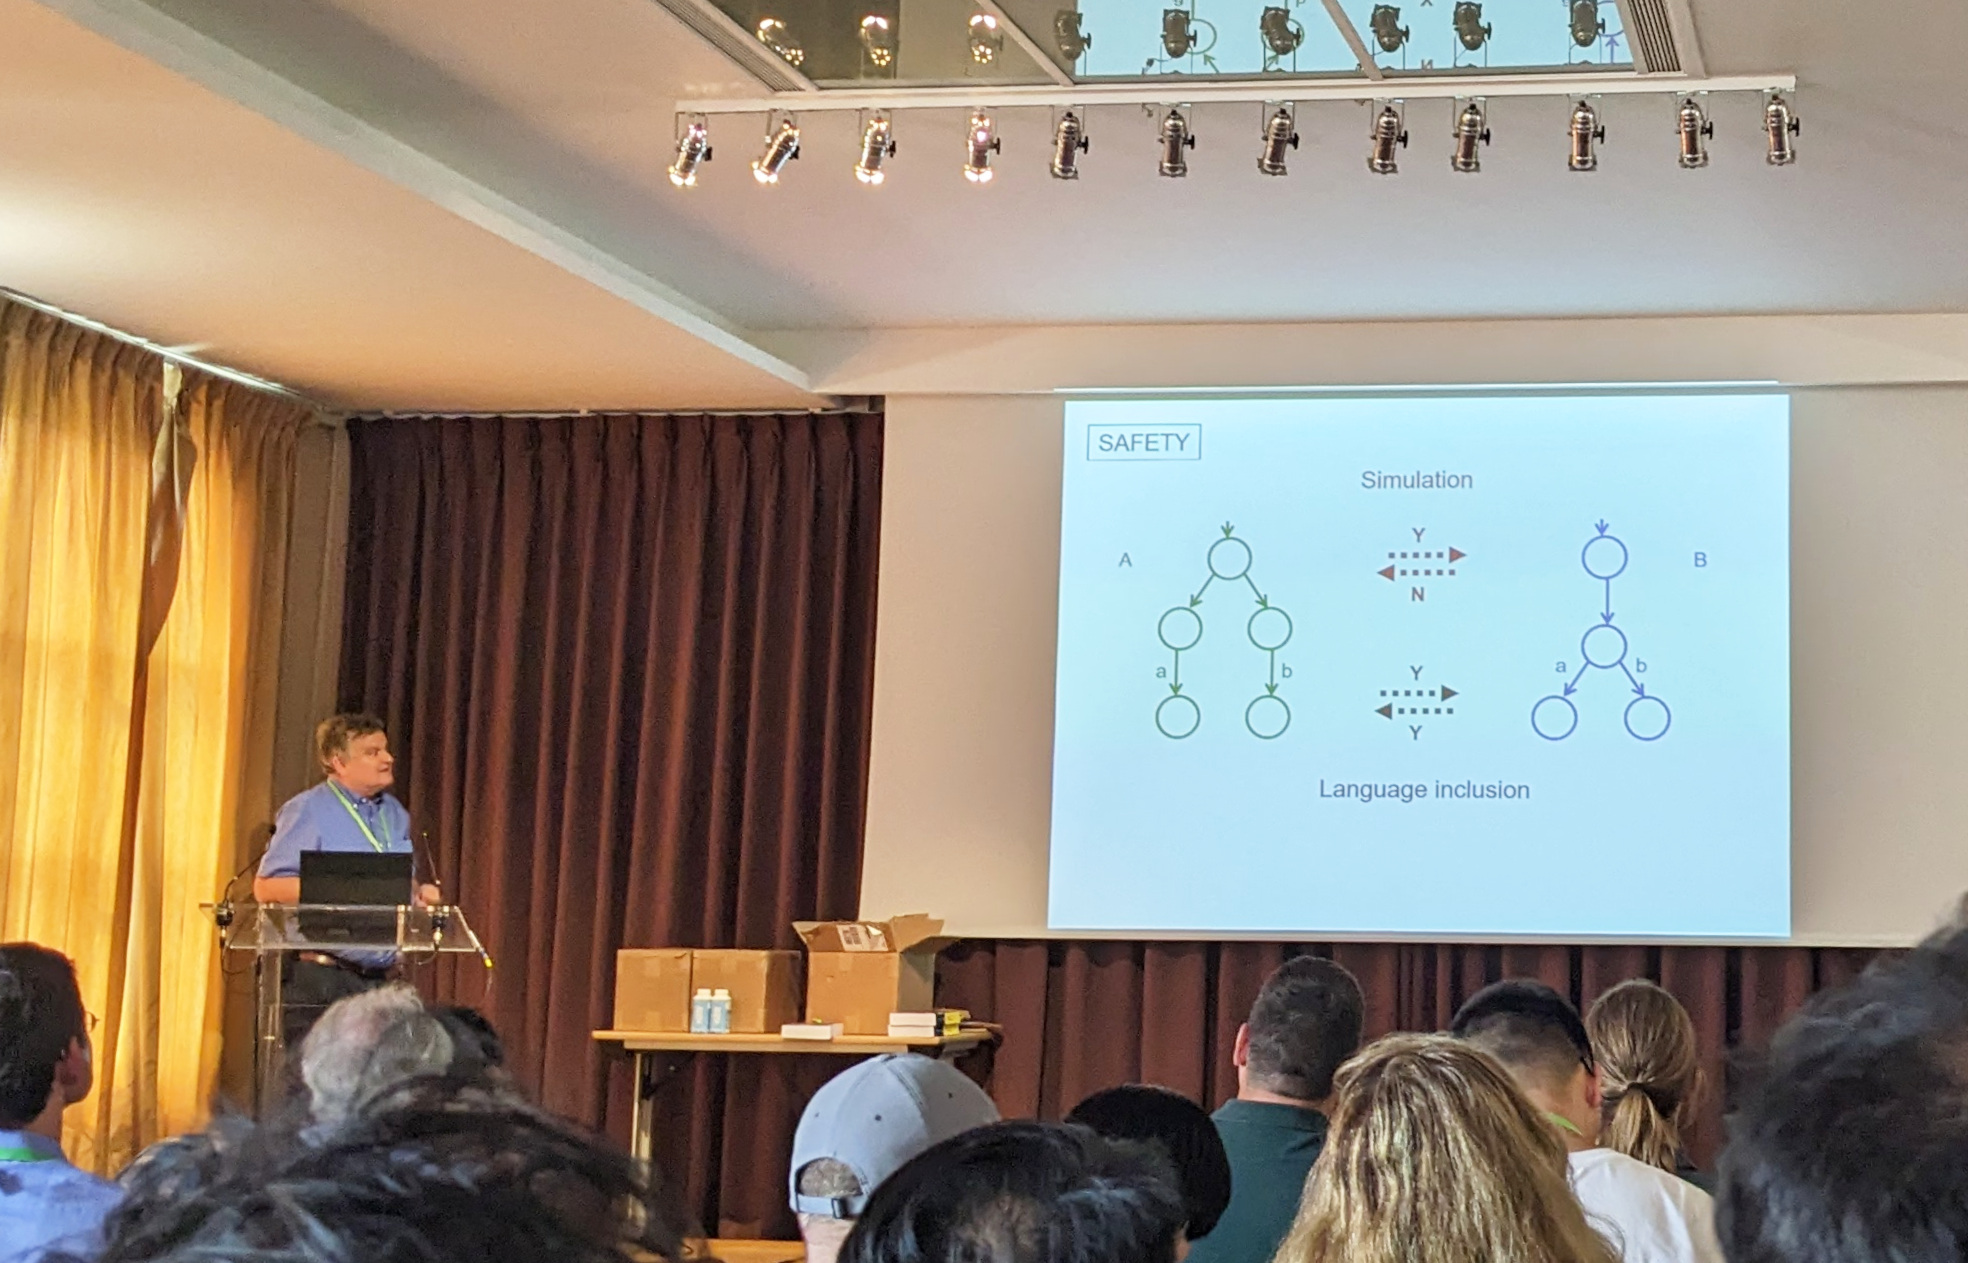
\includegraphics{img/henzinger.jpg}

}

\caption{\label{fig-henzinger}Tom Henzinger employing
Example~\ref{exm-ts} during CAV'23.}

\end{marginfigure}%

\begin{example}[A Classic
Example]\protect\hypertarget{exm-ts}{}\label{exm-ts}

Consider the transition system
\(\mathcal{S}_\mathsf{PQ} = (\{\mathsf{P}, \mathsf{p_a}, \mathsf{p_b}, \mathsf{p_1}, \mathsf{p_2}, \mathsf{Q}, \mathsf{q_{ab}}, \mathsf{q_1}, \mathsf{q_2}\}, \{\mathsf{a}, \mathsf{b}, τ\}, \xrightarrow{\cdot}_\mathsf{PQ})\)
given by the following graph:

\begin{figure}[H]

\centering{

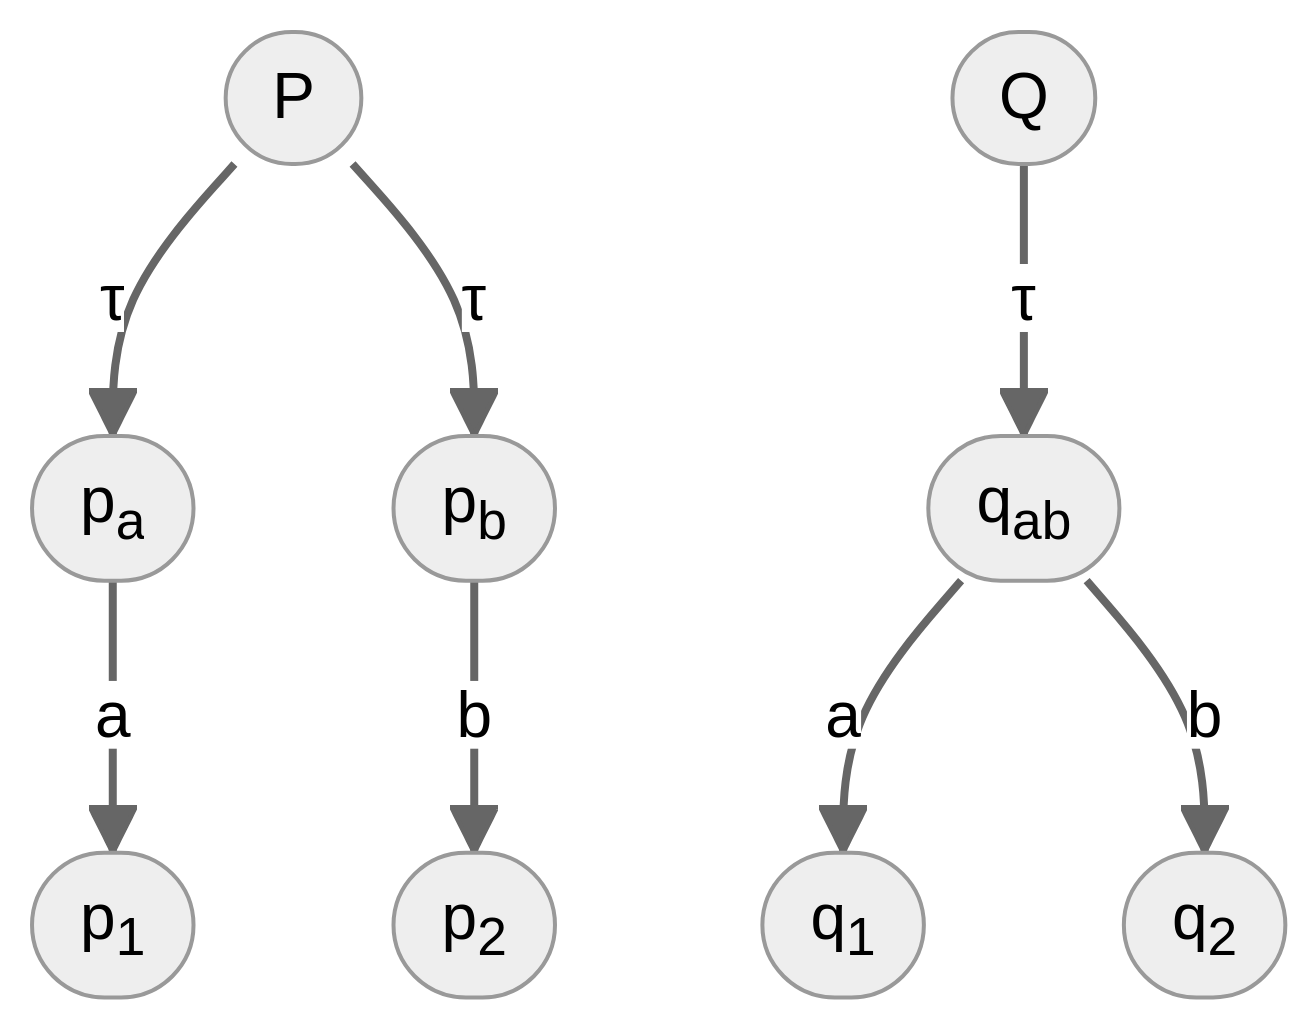
\includegraphics[width=3.43in,height=2.68in]{02_background_files/figure-latex/mermaid-figure-1.png}

}

\caption{\label{fig-ts-determinism}Example system
\(\mathcal{S}_\mathsf{PQ}\).}

\end{figure}%

\noindent  The program described by the transitions from \(\mathsf{P}\)
choses non-deterministically during a \(τ\)-step between two options and
then offers only either \(\mathsf{a}\) \emph{or} \(\mathsf{b}\). The
program \(\mathsf{Q}\) on the other hand performs a \(τ\)-step and then
offers the choice between options \(\mathsf{a}\) and \(\mathsf{b}\) to
the environment.

\end{example}

\noindent  There are two things one might wonder about
Example~\ref{exm-ts}:

\begin{enumerate}
\def\labelenumi{\arabic{enumi}.}
\tightlist
\item
  Should one care about non-determinism in programs? Subsection
  \ref{sec-ccs} shows how non-determinism arises naturally in concurrent
  programs.
\item
  Should one consider \(\mathsf{P}\) and \(\mathsf{Q}\) equivalent? This
  heavily depends. Section \ref{sec-behavioral-eq} will introduce a
  notion of equivalence under which the two are equivalent and one under
  which they differ.
\end{enumerate}

\subsection{Calculus of Communicating Systems}\label{sec-ccs}

To talk about programs in this thesis, we will use Milner's
\citeyearpar{milner1989comcon} \emph{Calculus of Communicating Systems}
(CCS).

\begin{definition}[Calculus of Communicating
Systems]\protect\hypertarget{def-ccs}{}\label{def-ccs}

Let \(\mathcal{A}\) be a set of channel names, and \(\mathcal X\) a set
of process names. Then, \(\textsf{CCS}\) processes, communicating via
actions
\(\Sigma_\textsf{CCS}≔ \mathcal{A}\cup \{ \overline{\alpha} \mid \alpha \in \mathcal{A}\} \cup \{τ\}\),
are given by the following grammar:

\[
  \begin{array}{cllr}
    P \;⩴\;
    & α\ldotp\! P & \quad\text{with } α ∈ \mathcal{A}&
        \text{“input action prefix”} \\
    & \overline{α}\ldotp\! P & \quad\text{with } α ∈ \mathcal{A}&
        \text{“output action prefix”} \\
    & τ\ldotp\! P & &
        \text{“internal action”} \\
    & \mathbf{0}& &
        \text{“null process”} \\
    & X & \quad\text{with } X ∈ \mathcal X&
        \text{“recursion”} \\
    & P +P & &
        \text{“choice”} \\
    & P \, \mid\, P & &
        \text{“parallel composition”} \\
    & P \, \mathbin{\backslash}A & \quad\text{with } A ⊆ \mathcal{A}&
        \text{“restriction”}
  \end{array}
  \] We call pairs of actions \(α\) and \(\overline{α}\)
\emph{coactions}, and work with the aliasing
\(\overline{\overline{α}} = α\). The intuition is that an action \(α\)
represents receiving and \(\overline{α}\) expresses sending in
communication. A pair of action and coaction can ``react'' in a
communication situation and only become internal activity \(τ\) in the
view of the environment.

Each sub-process tree must end in a \(\mathbf{0}\)-process or recursion.
For brevity, we usually drop a final \(\mathbf{0}\) when writing terms,
e.g., just writing \(\mathsf{ac}\) for
\(\mathsf{ac}\ldotp\! \mathbf{0}\).

We place parenthesis, \((…)\), in terms where the syntax trees are
otherwise ambiguous, but understand the choice operator \(+\) and the
parallel operator \(\mid\) to be associative.

\end{definition}

\begin{example}[Concurrent
Philosophers]\protect\hypertarget{exm-ccs}{}\label{exm-ccs}

Following tradition, we will express our examples in terms of
philosophers who need forks to eat spaghetti.\sidenote{\footnotesize  Of course, you
  can just as well read the examples to be about computer programs that
  race for resources.} So, consider two philosophers \(\mathsf{P_A}\)
and \(\mathsf{P_B}\) who want to grab a resource \(\mathsf{fork}\)
modeled as an action in order to eat where we express \(\mathsf{P_A}\)
eating with action \(\mathsf{a}\) and \(\mathsf{P_B}\) eating with
\(\mathsf{b}\). The philosopher processes read:

\marginnote{\begin{footnotesize}

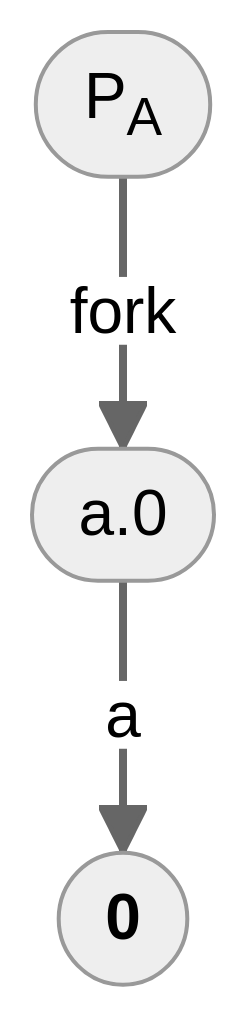
\includegraphics[width=0.64in,height=2.65in]{02_background_files/figure-latex/mermaid-figure-5.png}

\end{footnotesize}}

\[
  \begin{gathered}
    \mathsf{P_A} ≔ \mathsf{fork}\ldotp\! \mathsf{a}\ldotp\! \mathbf{0}\\
    \mathsf{P_B} ≔ \mathsf{fork}\ldotp\! \mathsf{b}\ldotp\! \mathbf{0}
  \end{gathered}
  \] An LTS representation of \(\mathsf{P_A}\)'s behavior can be seen in
the margin. Process \(\mathsf{P}\) captures the whole scenario where the
two philosophers compete for the fork using communication: \[
    \mathsf{P} ≔ ( \overline{\mathsf{fork}}\ldotp\! \mathbf{0}\mid\mathsf{P_A} \mid\mathsf{P_B} ) \mathbin{\backslash}\{\mathsf{fork}\}
  \] The restriction \(… \mathbin{\backslash}\{\mathsf{fork}\}\)
expresses that the \(\mathsf{fork}\)-channel can only be used for
communication within the system.

As the \(\overline{\mathsf{fork}}\)-action can be consumed by just one
of the two philosophers, process \(\mathsf{P}\) expresses exactly the
program behavior seen in state \(\mathsf{P}\) of Example~\ref{exm-ts}.

\end{example}

\noindent  The formal relationship between process terms and their LTS
semantics is given by the following definition.

\begin{definition}[CCS
Semantics]\protect\hypertarget{def-ccs-semantics}{}\label{def-ccs-semantics}

Given an assignment of names to processes,
\(\mathcal V\colon \mathcal X→ \textsf{CCS}\), the operational semantics
\({\xrightarrow{\cdot}_\textsf{CCS}} ⊆ \textsf{CCS}× \Sigma_\textsf{CCS}× \textsf{CCS}\)
is defined inductively by the rules:

\[
\dfrac{
}{
  α\ldotp\! P \xrightarrow{α}_\textsf{CCS}P
}
\qquad
\dfrac{
  P \xrightarrow{α}_\textsf{CCS}P' \qquad \mathcal V(X) = P
}{
  X \xrightarrow{α}_\textsf{CCS}P'
}
\]

\[
\dfrac{
  P_1 \xrightarrow{α}_\textsf{CCS}P_1'
}{
  P_1 +P_2 \xrightarrow{α}_\textsf{CCS}P_1'
}\qquad
\dfrac{
  P_2 \xrightarrow{α}_\textsf{CCS}P_2'
}{
  P_1 +P_2 \xrightarrow{α}_\textsf{CCS}P_2'
}
\]

\[
\dfrac{
  P_1 \xrightarrow{α}_\textsf{CCS}P_1'
}{
  P_1 \mid P_2 \xrightarrow{α}_\textsf{CCS}P_1' \mid P_2
}\qquad
\dfrac{
  P_2 \xrightarrow{α}_\textsf{CCS}P_2'
}{
  P_1 \mid P_2 \xrightarrow{α}_\textsf{CCS}P_1 \mid P_2'
}
\]

\[
\dfrac{
  P_1 \xrightarrow{α}_\textsf{CCS}P_1' \qquad
  P_2 \xrightarrow{\overline{α}}_\textsf{CCS}P_2'
}{
  P_1 \mid P_2 \xrightarrow{τ}_\textsf{CCS}P_1' \mid P_2'
}\qquad
\dfrac{
  P \xrightarrow{α}_\textsf{CCS}P' \qquad
  α, \overline{α} \notin A
}{
  P \mathbin{\backslash}A \xrightarrow{α}_\textsf{CCS}P' \mathbin{\backslash}A
}
\] A process \(P ∈ \textsf{CCS}\) now denotes a position in the
transition system
\((\textsf{CCS}, \Sigma_\textsf{CCS}, \xrightarrow{}_\textsf{CCS})\)
defined through Definition~\ref{def-ccs}.

\end{definition}

\noindent  Feel free to go ahead an check that the transitions of
Example~\ref{exm-ts} indeed match those that
Definition~\ref{def-ccs-semantics} prescribes for \(\mathsf{P}\) of
Example~\ref{exm-ccs}! (For readability, Example~\ref{exm-ts}, has
shorter state names, however.) For instance, the transition
\(\mathsf{P} \xrightarrow{τ} \mathsf{p_a}\) of Example~\ref{exm-ts}
would be justified as follows:

\[
\dfrac{
  \dfrac{
    \dfrac{
      \dfrac{
        \vphantom{\xrightarrow{\overline{\mathsf{fork}}}_\textsf{CCS}}
      }{
        \overline{\mathsf{fork}} \xrightarrow{\overline{\mathsf{fork}}}_\textsf{CCS}\mathbf{0}
      }
      \quad
      \dfrac{
        \dfrac{
          \overline{
            \mathsf{fork}\ldotp\! \mathsf{a}
            \xrightarrow{\mathsf{fork}}_\textsf{CCS}
            \mathsf{a}
          }
          \qquad
          \mathcal V(\mathsf{P_A}) = \mathsf{fork}\ldotp\! \mathsf{a}
        }{
          \mathsf{P_A} \xrightarrow{\mathsf{fork}}_\textsf{CCS}\mathsf{a}
        }
      }{
        \mathsf{P_A} \mid\mathsf{P_B} \xrightarrow{\mathsf{fork}}_\textsf{CCS}\mathsf{a} \mid\mathsf{P_B}
      }
    }{
      \overline{\mathsf{fork}} \mid\mathsf{P_A} \mid\mathsf{P_B}
      \xrightarrow{τ}_\textsf{CCS}
      \mathbf{0}\mid\mathsf{a} \mid\mathsf{P_B}
    }
    \quad
    \begin{matrix}
      \vphantom{\xrightarrow{\overline{\mathsf{fork}}}_\textsf{CCS}}\\
      τ \notin A
    \end{matrix}
  }{
    ( \overline{\mathsf{fork}} \mid\mathsf{P_A} \mid\mathsf{P_B} ) \mathbin{\backslash}\{\mathsf{fork}\}
    \xrightarrow{τ}_\textsf{CCS}
    ( \mathbf{0}\mid\mathsf{a} \mid\mathsf{P_B} ) \mathbin{\backslash}\{\mathsf{fork}\}
  }
  \quad
  \begin{matrix}
    \vphantom{\xrightarrow{\overline{\mathsf{fork}}}_\textsf{CCS}}\\
    \mathcal V(\mathsf{P}) = ( \overline{\mathsf{fork}} \mid\mathsf{P_A} \mid\mathsf{P_B} ) \mathbin{\backslash}\{\mathsf{fork}\}
  \end{matrix}
}{
  \mathsf{P} \xrightarrow{τ}_\textsf{CCS}( \mathbf{0}\mid\mathsf{a} \mid\mathsf{P_B} ) \mathbin{\backslash}\{\mathsf{fork}\}
}
\]

\noindent  Non-determinism like in \(\mathsf{P}\) of
Example~\ref{exm-ts} can be understood as a natural phenomenon in models
with concurrency. The model leaves unspecified which of two processes
will consume an internal resource and, to the outsider, it is
transparent which one took the resource until they communicate. There
are other ways how non-determinism plays a crucial role in models, for
instance, as consequence of abstraction or parts that are left open in
specifications.

The second process \(\mathsf{Q}\) of Example~\ref{exm-ts} can be
understood as a deterministic sibling of \(\mathsf{P}\).

\begin{example}[Deterministic
Philosophers]\protect\hypertarget{exm-deterministic-phil}{}\label{exm-deterministic-phil}

A process matching the transitions from \(\mathsf{Q}\) in
Example~\ref{exm-ts} would be the following, where the philosophers take
the fork as a team and then let the environment choose who of them eats:

\[
\mathsf{Q} ≔ (\overline{\mathsf{fork}} \mid\mathsf{fork}\ldotp\! ( \mathsf{a} +\mathsf{b} )) \mathbin{\backslash}\{\mathsf{fork}\}.
\]

\end{example}

\section{Behavioral Equivalences}\label{sec-behavioral-eq}

\subsection{Trace Equivalence}\label{trace-equivalence}

\begin{definition}[Traces]\protect\hypertarget{def-traces}{}\label{def-traces}

The set of traces of a process \(\mathsf{Traces}(p)\) is recursively
defined as

\begin{itemize}
\tightlist
\item
  \(\texttt{()}∈ \mathsf{Traces}(p)\),\sidenote{\footnotesize We denote the empty word
    by \(\texttt{()}\).}
\item
  \(α \cdot \vec w ∈ \mathsf{Traces}(p)\) if there is \(p'\) with
  \(p \xrightarrow{α} p'\) and \(\vec w ∈ \mathsf{Traces}(p')\).
\end{itemize}

\end{definition}

\begin{definition}[Trace
Equivalence]\protect\hypertarget{def-trace-eq}{}\label{def-trace-eq}

Two processes \(p\) and \(q\) are considered \emph{trace-equivalent},
written \(p \sim_\mathrm{T} q\), if
\(\mathsf{Traces}(p) = \mathsf{Traces}(q)\).

Processes are \emph{trace-preordered}, \(p \preceq_\mathrm{T} q\), if
\(\mathsf{Traces}(p) ⊆ \mathsf{Traces}(q)\).

\end{definition}

\begin{example}[]\protect\hypertarget{exm-phil-traces}{}\label{exm-phil-traces}

The traces for the processes of Example~\ref{exm-ts} would be
\(\mathsf{Traces}(\mathsf{P}) = \{\texttt{()}, τ, τ\mathsf{a}, τ\mathsf{b}\} = \mathsf{Traces}(\mathsf{Q})\).
Consequently, \(\mathsf{P}\) and \(\mathsf{Q}\) are trace-equivalent,
\(\mathsf{P} \sim_\mathrm{T} \mathsf{Q}\).

As
\(\mathsf{Traces}(\mathsf{p_a}) = \{\texttt{()}, \mathsf{a}\} ⊆ \{\texttt{()}, \mathsf{a}, \mathsf{b}\} = \mathsf{Traces}(\mathsf{q_{ab}})\),
\(\mathsf{p_a}\) is trace-preordered to \(\mathsf{q_{ab}}\),
\(\mathsf{p_a} \preceq_\mathrm{T} \mathsf{q_{ab}}\). This ordering is
strict, that is,
\(\mathsf{q_{ab}} \not\preceq_\mathrm{T} \mathsf{p_a}\), due to
\(\mathsf{b} ∈ \mathsf{Traces}(\mathsf{q_{ab}})\) but
\(\mathsf{b} \notin \mathsf{Traces}(\mathsf{p_a})\). We could say that
trace \(\mathsf{b}\) constitutes a \emph{difference} between
\(\mathsf{q_{ab}}\) and \(\mathsf{p_a}\).

\end{example}

\begin{proposition}[]\protect\hypertarget{prp-trace-eq-rel}{}\label{prp-trace-eq-rel}

The trace preorder \(\preceq_\mathrm{T}\) is indeed a preorder (i.e.,
transitive and reflexive) and trace equivalence \(\sim_\mathrm{T}\) is
indeed an equivalence relation (i.e., transitive, reflexive, and
moreover symmetric).

\end{proposition}

\begin{proof}
The properties carry over directly from \(⊆\) and \(=\) on sets of
\(\mathsf{Traces}(\cdot)\).
\end{proof}

\subsection{Simulation and
Bisimulation}\label{simulation-and-bisimulation}

\begin{definition}[Simulation]\protect\hypertarget{def-simulation}{}\label{def-simulation}

A relation on states, \(\mathcal{R} ⊆ \mathcal{P}× \mathcal{P}\), is
called a \emph{simulation} if, for each \((p, q) ∈ \mathcal{R}\) and
\(α ∈ \Sigma\) with \(p \xrightarrow{a} p'\) there is a \(q'\) with
\(q \xrightarrow{α} q'\) and \((p', q') ∈ \mathcal{R}\).

\end{definition}

\begin{definition}[(Bi-)similarity]\protect\hypertarget{def-bisimilarity}{}\label{def-bisimilarity}

Simulation-preorder, similarity and bisimilarity are defined as follows:

\begin{itemize}
\tightlist
\item
  \(p\) is \emph{simulated by} \(q\), \(p \preceq_\mathrm{S} q\), iff
  there is a simulation \(\mathcal{R}\) with \((p, q) ∈ \mathcal{R}\).
\item
  \(p\) is \emph{similar} to \(q\), \(p \sim_\mathrm{S} q\), iff
  \(p \preceq_\mathrm{S} q\) and \(q \preceq_\mathrm{S} p\).
\item
  \(p\) is \emph{bisimilar} to \(q\), \(p \sim_\mathrm{B} q\), iff there
  is a \emph{symmetric} simulation \(\mathcal{R}\)
  (i.e.~\(\mathcal{R} = \mathcal{R}^{-1}\)) with
  \((p, q) ∈ \mathcal{R}\).
\end{itemize}

\end{definition}

\begin{example}[]\protect\hypertarget{exm-phil-sim}{}\label{exm-phil-sim}

The following relations are simulations on the LTS of
Example~\ref{exm-ts}:

\begin{itemize}
\tightlist
\item
  the empty relation \(\mathcal{R}_\varnothing ≔ \varnothing\);
\item
  the identity relation
  \(\mathcal{R}_\mathrm{id} ≔ \mathrm{id}_{\{\mathsf{P}, \mathsf{p_a}, \mathsf{p_b}, \mathsf{p_1}, \mathsf{p_2}, \mathsf{Q}, \mathsf{q_{ab}}, \mathsf{q_1}, \mathsf{q_2}\}} = \{(\mathsf{P}, \mathsf{P}),\allowbreak (\mathsf{p_a}, \mathsf{p_a}),\allowbreak (\mathsf{p_b}, \mathsf{p_b}), (\mathsf{p_1}, \mathsf{p_1}),\allowbreak (\mathsf{p_2}, \mathsf{p_2}), (\mathsf{Q}, \mathsf{Q}), (\mathsf{q_{ab}}, \mathsf{q_{ab}}), \allowbreak(\mathsf{q_1}, \mathsf{q_1}), (\mathsf{q_2}, \mathsf{q_2})\}\);
\item
  the universal relation between all final states
  \(\mathcal{R}_\mathrm{fin} ≔ \{\mathsf{p_1}, \mathsf{p_2}, \mathsf{q_1}, \mathsf{q_2}\}²\),
\item
  more generally, the relation from final states to all other states:
  \(\mathcal{R}_\mathrm{up} ≔ \{\mathsf{p_1}, \mathsf{p_2}, \mathsf{q_1}, \mathsf{q_2}\} × \mathcal{P}\);
\item
  a minimal simulation for \(\mathsf{P}\) and \(\mathsf{Q}\):
  \(\mathcal{R}_\mathsf{PQ} ≔ \{(\mathsf{P}, \mathsf{Q}), (\mathsf{p_a}, \mathsf{q_{ab}}), (\mathsf{p_b}, \mathsf{q_{ab}}), (\mathsf{p_1}, \mathsf{q_1}), (\mathsf{p_2}, \mathsf{q_2})\}\);
\item
  and the combination of the above
  \(\mathcal{R}_\mathrm{max} ≔ \mathcal{R}_\mathrm{sim} ∪ \mathcal{R}_\mathrm{id} ∪ \mathcal{R}_\mathrm{up}\).
\end{itemize}

\noindent  The simulation \(\mathcal{R}_\mathsf{PQ}\) shows that
\(\mathsf{P} \preceq_\mathrm{S} \mathsf{Q}\).

However, there is no simulation that preorders \(\mathsf{Q}\) to
\(\mathsf{P}\), as there is no way to simulate the transition
\(\mathsf{Q} \xrightarrow{τ} \mathsf{q_{ab}}\) from \(\mathsf{P}\) for
lack of a successor that allows \(\mathsf{a}\) \emph{and} \(\mathsf{b}\)
as does \(\mathsf{q_{ab}}\). (In Section~\ref{sec-hml}, we will discuss
how to capture such differences more formally.)

Thus, \(\mathsf{Q} \not\preceq_\mathrm{S} \mathsf{P}\), and
\(\mathsf{P} \nsim_\mathrm{S} \mathsf{Q}\). Moreover, there cannot be a
symmetric simulation, \(\mathsf{P} \nsim_\mathrm{B} \mathsf{Q}\).

\end{example}

\begin{proposition}[]\protect\hypertarget{prp-sim-eq-rel}{}\label{prp-sim-eq-rel}

The simulation preorder \(\preceq_\mathrm{S}\) is indeed a preorder and
\(\sim_\mathrm{S}\) and \(\sim_\mathrm{B}\) are equivalences.

\end{proposition}

\begin{proof}
\leavevmode

\begin{enumerate}
\def\labelenumi{\arabic{enumi}.}
\tightlist
\item
  Reflexivity of \(\preceq_\mathrm{S}\), \(\sim_\mathrm{S}\) and
  \(\sim_\mathrm{B}\): \(\mathrm{id}_{\mathcal{P}}\) is a (symmetric)
  simulation on each transition system.
\item
  Transitivity of \(\preceq_\mathrm{S}\): If \(\mathcal{R}_1\) and
  \(\mathcal{R}_2\) are simulations, then the composition
  \(\mathcal{R}_1 \circ \mathcal{R}_2\) too is a simulation. This also
  establishes transitivity of \(\sim_\mathrm{S}\) and
  \(\sim_\mathrm{B}\).
\item
  Symmetry of \(\sim_\mathrm{S}:\) By definition.
\item
  Symmetry of \(\sim_\mathrm{B}\): \(p \sim_\mathrm{B} q\) implies there
  is a symmetric simulation \(\mathcal{R}\) with
  \((p,q) \in \mathcal{R}\). As \(\mathcal{R} = \mathcal{R}^{-1}\), this
  implies \((q,p) \in \mathcal{R}\) and thus \(q \sim_\mathrm{B} p\).
\end{enumerate}

\end{proof}

\subsection{The Hierarchy of
Equivalences}\label{the-hierarchy-of-equivalences}

Bisimilarity, similarity and trace equivalence form a small hierarchy of
equivalences in the sense that they imply one-another in one direction,
but not in the other. Let us quickly make this formal:

\begin{marginfigure}

\centering{

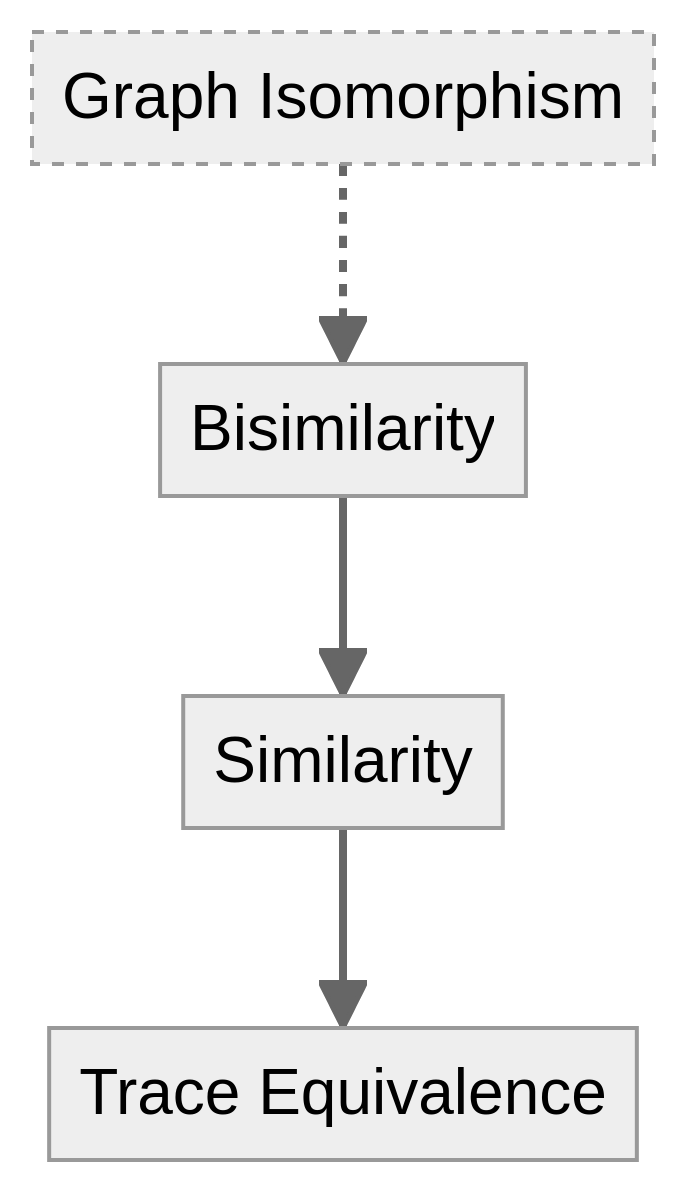
\includegraphics[width=1.79in,height=3.1in]{02_background_files/figure-latex/mermaid-figure-4.png}

}

\caption{\label{fig-core-hierarchy}Core hierarchy of equivalences.}

\end{marginfigure}%

\begin{lemma}[]\protect\hypertarget{lem-bisim-bisim}{}\label{lem-bisim-bisim}

The relation \(\sim_\mathrm{B}\) is itself a symmetric simulation.

\end{lemma}

\begin{corollary}[]\protect\hypertarget{cor-bisim-impl-sim}{}\label{cor-bisim-impl-sim}

If \(p \sim_\mathrm{B} q\), then \(p \sim_\mathrm{S} q\).

\end{corollary}

\begin{lemma}[]\protect\hypertarget{lem-sim-impl-traces}{}\label{lem-sim-impl-traces}

If \(p \preceq_\mathrm{S} q\), then \(p \preceq_\mathrm{T} q\).
(Consequently, \(p \sim_\mathrm{S} q\) also implies
\(p \sim_\mathrm{T} q\).)

\end{lemma}

\noindent  We also have seen with example Example~\ref{exm-phil-sim}
that this hierarchy is strict between trace and simulation preorder in
the sense that there exist \(p,q\) with \(p \preceq_\mathrm{T} q\) but
not \(p \preceq_\mathrm{S} q\). The hierarchy also is strict between
similarity and bisimilarity as the following example shows.

\begin{example}[Trolled
philosophers]\protect\hypertarget{exm-bisim-sim}{}\label{exm-bisim-sim}

Let us extend Example~\ref{exm-deterministic-phil} with a troll process
that might consume the \(\mathsf{fork}\) and then do nothing: \[
  \mathsf{Q'} ≔ (\overline{\mathsf{fork}} \mid\mathsf{fork} \mid\mathsf{fork}\ldotp\! ( \mathsf{a} +\mathsf{b} )) \mathbin{\backslash}\{\mathsf{fork}\}.
  \] This adds another deadlock state to the transition system, seen in
Figure~\ref{fig-bisim-sim-ts}.

\begin{marginfigure}

\centering{

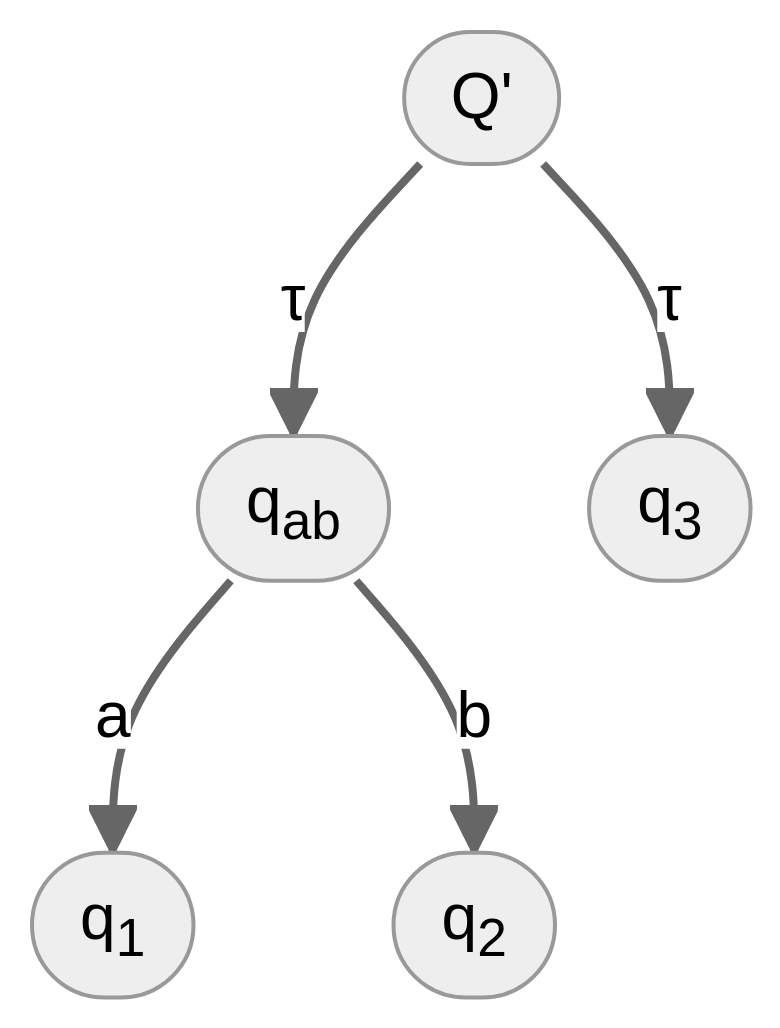
\includegraphics[width=2.04in,height=2.68in]{02_background_files/figure-latex/mermaid-figure-3.png}

}

\caption{\label{fig-bisim-sim-ts}Example with new deadlock
\(\mathsf{q_3}\).}

\end{marginfigure}%

To similarity, this change is invisible, that is
\(\mathsf{Q} \sim_\mathrm{S} \mathsf{Q'}\). (Reason: The relation
\(\{(\mathsf{Q}, \mathsf{Q'}), (\mathsf{Q'}, \mathsf{Q})\} \cup \mathrm{id}_{\{ \mathsf{q_{ab}}, \mathsf{q_1}, \mathsf{q_2}, \mathsf{q_3}\}}\)
is a simulation.)

However, to bisimilarity, \(\mathsf{Q'} \xrightarrow{τ} \mathsf{q_3}\)
constitutes a difference. There cannot be a symmetric simulation
handling this transition as \(\mathsf{Q}\) has no deadlocked successors.
Thus \(\mathsf{Q} \nsim_\mathrm{B} \mathsf{Q'}\).

\end{example}

The equivalences we have been discussed so far could also be understood
as abstractions of an even finer equivalence, namely graph isomorphism:

\begin{definition}[Graph
Isomorphism]\protect\hypertarget{def-graph-isomorphism}{}\label{def-graph-isomorphism}

A bijective function \(\mathcal{f} \colon \mathcal{P}\to \mathcal{P}\)
is called a \emph{graph isomorphism} on a transition system if, for all
\(p,p', α\), the transition \(p \xrightarrow{α} p'\) exists if and only
if the transition \(\mathcal{f}(p) \xrightarrow{α} \mathcal{f}(p')\)
exists.

Two states \(p\) and \(q\) are considered
\emph{graph-isomorphism-equivalent}, \(p \sim_\mathrm{GI} q\), iff there
is a graph isomorphism \(\mathcal{f}\) with \(\mathcal{f}(p) = q\).

\end{definition}

\begin{example}[]\protect\hypertarget{exm-graph-isomorphism}{}\label{exm-graph-isomorphism}

Consider the transition system in Figure~\ref{fig-iso-ts}.
\(\mathsf{p_{even}} \sim_\mathrm{GI} \mathsf{p_{odd}}\) because
\(\mathcal{f} ≔ \{\mathsf{p_{even}} \mapsto \mathsf{p_{odd}}, \mathsf{p_{odd}} \mapsto \mathsf{p_{even}}\}\)
is a graph isomorphism.

\begin{marginfigure}

\centering{

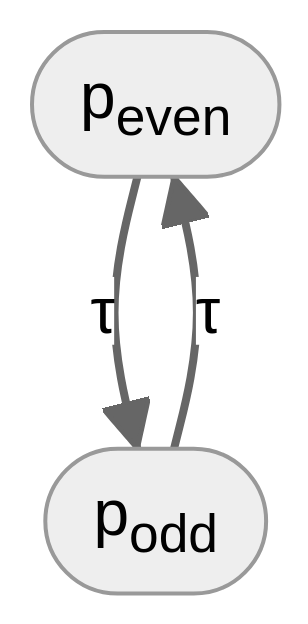
\includegraphics[width=0.81in,height=1.63in]{02_background_files/figure-latex/mermaid-figure-2.png}

}

\caption{\label{fig-iso-ts}Transition system with an isomorphic cycle.}

\end{marginfigure}%

\end{example}

\begin{lemma}[]\protect\hypertarget{lem-iso-impl-bisim}{}\label{lem-iso-impl-bisim}

The relation \(\sim_\mathrm{GI}\) is itself a symmetric simulation and
thus \(p \sim_\mathrm{GI} q\) implies \(p \sim_\mathrm{B} q\).

\end{lemma}

Once again, the hierarchy is strict because of bisimilarity being less
restricted in the matching of equivalent states.

\begin{example}[]\protect\hypertarget{exm-iso-vs-bisim}{}\label{exm-iso-vs-bisim}

Consider the processes
\(\mathsf{P_1} ≔ (\overline{\mathsf{fork}} \mid\mathsf{fork}) \mathbin{\backslash}\{\mathsf{fork}\}\)
and
\(\mathsf{P_2} ≔ (\overline{\mathsf{fork}} \mid\mathsf{fork} \mid\mathsf{fork}) \mathbin{\backslash}\{\mathsf{fork}\}\).
\(\mathsf{P_1}\) can transition to
\((\mathbf{0}\mid\mathbf{0}) \mathbin{\backslash}\{\mathsf{fork}\}\),
while \(\mathsf{P_2}\) has two options, namely
\((\mathbf{0}\mid\mathbf{0}\mid\mathsf{fork}) \mathbin{\backslash}\{\mathsf{fork}\}\)
and
\((\mathbf{0}\mid\mathsf{fork} \mid\mathbf{0}) \mathbin{\backslash}\{\mathsf{fork}\}\).
All three reachable processes are deadlocks and thus isomorphic. But
\(\mathsf{P_1} \nsim_\mathrm{GI} \mathsf{P_2}\) because no bijection can
connect the one successor of \(\mathsf{P_1}\) and the two of
\(\mathsf{P_2}\). However,
\(\mathsf{P_1} \sim_\mathrm{B} \mathsf{P_2}\), as bisimilarity is more
relaxed.

\end{example}

\section{Observations as Modal Logic}\label{sec-hml}

\subsection{Hennessy--Milner Logic to Express
Observations}\label{hennessymilner-logic-to-express-observations}

\begin{definition}[Hennessy--Milner
Logic]\protect\hypertarget{def-hml}{}\label{def-hml}

Formulas of \emph{Hennessy--Milner logic} \(\textsf{HML}\) are given by
the grammar:

\[
\begin{array}{rcllr}
  φ & \;⩴\;&
    \langle α \rangle φ & \quad\text{with } α ∈ \Sigma&
      \text{“observation”} \\
    & \;\mid\;& \textstyle\bigwedge_{i \in I}φ_i & \quad\text{with index set } I & \text{“conjunction”} \\
    & \;\mid\;& \neg φ & & \text{“negation”} \\
\end{array}
\]

\end{definition}

\noindent  We also write conjunctions as sets
\(\textstyle\bigwedge \{φ_1, φ_2…\}\). The empty conjunction
\(\textstyle\bigwedge \varnothing\) is denoted by \(\top\) and serves as
the nil-element of HML syntax trees. We also usually omit them when
writing down formulas, e.g., shortening
\(\langle \mathsf{a} \rangle\langle \mathsf{b} \rangle\top\) to
\(\langle \mathsf{a} \rangle\langle \mathsf{b} \rangle\).

The intuition behind HML is that it describes \emph{what sequences of
behavior} one may or may not \emph{observe} of a system. Observations
\(\langle α \rangle…\) are used to build up possible action sequences;
conjunctions \(\textstyle\bigwedge \{…\}\) capture branching points in
decision trees; and negations \(\neg…\) describe impossibilities.

\begin{definition}[HML
semantics]\protect\hypertarget{def-hml-semantics}{}\label{def-hml-semantics}

The semantics of HML
\(\llbracket \cdot \rrbracket \colon \textsf{HML}→ 2^{\mathcal{P}}\) is
defined recursively by:

\[
\begin{array}{rcl}
  \llbracket \langle α \rangle φ \rrbracket & ≔ & \{p \mid \exists p' ∈ \llbracket φ \rrbracket \ldotp p \xrightarrow{α} p'\},\\
  \llbracket \textstyle\bigwedge_{i \in I}φ_i \rrbracket & ≔ & \bigcap_{i ∈ I} \llbracket φ_i \rrbracket,\\
  \llbracket \neg φ \rrbracket & ≔ & \mathcal{P}\mathbin{\backslash}\llbracket φ \rrbracket.
\end{array}
\]

\end{definition}

\begin{example}[]\protect\hypertarget{exm-hml}{}\label{exm-hml}

Let us consider some observations on the system of Example~\ref{exm-ts}.

\begin{itemize}
\tightlist
\item
  \(\llbracket \langle τ \rangle\langle \mathsf{a} \rangle \rrbracket = \{\mathsf{P}, \mathsf{Q}\}\)
  as both, \(\mathsf{P}\) and \(\mathsf{Q}\), expose the trace
  \(τ\mathsf{a}\),
\item
  \(\mathsf{Q} ∈ \llbracket \langle τ \rangle\textstyle\bigwedge \{\langle \mathsf{a} \rangle, \langle \mathsf{b} \rangle\} \rrbracket\),
  but
  \(\mathsf{P} \notin \llbracket \langle τ \rangle\textstyle\bigwedge \{\langle \mathsf{a} \rangle, \langle \mathsf{b} \rangle\} \rrbracket\).
\item
  \(\mathsf{P} ∈ \llbracket \langle τ \rangle\neg\langle \mathsf{a} \rangle \rrbracket\),
  but
  \(\mathsf{Q} \notin \llbracket \langle τ \rangle\neg\langle \mathsf{a} \rangle \rrbracket\).
\end{itemize}

\end{example}

\subsection{Characterizing Bisimilarity via
HML}\label{characterizing-bisimilarity-via-hml}

\begin{definition}[Distinctions and
Equivalences]\protect\hypertarget{def-distinctions}{}\label{def-distinctions}

We say that formula \(φ ∈ \textsf{HML}\) \emph{distinguishes} state
\(p\) \emph{from} state \(q\) if \(p ∈ \llbracket φ \rrbracket\) but
\(q \notin \llbracket φ \rrbracket\).

We say a sublogic \(\mathcal{O}_{X} ⊆ \textsf{HML}\) \emph{preorders}
state \(p\) to \(q\), \(p \preceq_{\mathcal{O}_{X}} q\), if no
\(φ ∈ \mathcal{O}_{X}\) is distinguishing \(p\) from \(q\). If the
preordering goes in both directions, we say that \(p\) and \(q\) are
equivalent with respect to sublogic \(\mathcal{O}_{X}\), written
\(p \sim_{\mathcal{O}_{X}} q\).

\end{definition}

\noindent  By this account,
\(\langle τ \rangle\neg\langle \mathsf{a} \rangle\) of
Example~\ref{exm-hml} distinguishes \(\mathsf{P}\) from \(\mathsf{Q}\).
\(\langle τ \rangle\textstyle\bigwedge \{\langle \mathsf{a} \rangle, \langle \mathsf{b} \rangle\}\),
on the other hand, distinguishes \(\mathsf{Q}\) from \(\mathsf{P}\).
(The direction matters!) For instance, the sublogic
\(\{\langle τ \rangle\langle \mathsf{a} \rangle, \langle τ \rangle\langle \mathsf{b} \rangle\}\)
preorders \(\mathsf{P}\) and \(\mathsf{Q}\) in both directions; so the
two states are equivalent with respect to this logic.

\begin{proposition}[]\protect\hypertarget{prp-hml-eq}{}\label{prp-hml-eq}

Consider an arbitrary HML sublogic \(\mathcal{O}_{X} ⊆ \textsf{HML}\).
Then, \(\preceq_{\mathcal{O}_{X}}\) is a preorder, and
\(\sim_{\mathcal{O}_{X}}\) an equivalence relation.

\end{proposition}

\begin{lemma}[]\protect\hypertarget{lem-hml-eq-sim}{}\label{lem-hml-eq-sim}

Hennessy--Milner logic equivalence \(\sim_{\textsf{HML}}\) is a
simulation relation.

\end{lemma}

\begin{proof}
Assume it were not. Then there would need to be
\(p \sim_{\textsf{HML}} q\) with step \(p \xrightarrow{\alpha }p'\), and
no \(q'\) such that \(q \xrightarrow{α} q'\) and
\(p' \sim_{\textsf{HML}} q'\). So there would need to be a
distinguishing formula \(φ_{q'}\) for each \(q'\) that \(q\) can reach
by an \(α\)-step. Consider the formula
\(φ_α ≔ \langle α \rangle\textstyle\bigwedge_{q' \in \{q' \mid q \xrightarrow{α} q'\}} φ_{q'}\).
It must be true for \(p\) and false for \(q\), contradicting
\(p \sim_{\textsf{HML}} q\).
\end{proof}

\begin{lemma}[HML Bisimulation
Invariance]\protect\hypertarget{lem-hml-eq-bisim-invariant}{}\label{lem-hml-eq-bisim-invariant}

If \(p \in \llbracket φ \rrbracket\) and \(p \sim_\mathrm{B} q\) then
\(q \in \llbracket φ \rrbracket\).

\end{lemma}

\begin{proof}
Induct over the structure of \(φ\) with arbitrary \(p\) and \(q\).

\begin{itemize}
\tightlist
\item
  Case \(p ∈ \llbracket \langle α \rangle φ \rrbracket\). Thus there is
  \(p' ∈ \llbracket φ \rrbracket\) with \(p \xrightarrow{α} p'\).
  Because \(\sim_\mathrm{B}\) is a simulation according to
  Lemma~\ref{lem-bisim-bisim}, this implies \(q'\) with
  \(p' \sim_\mathrm{B} q'\). The induction hypothesis makes
  \(p' ∈ \llbracket φ \rrbracket\) entail
  \(q' ∈ \llbracket φ \rrbracket\) and thus
  \(q ∈ \llbracket \langle α \rangle φ \rrbracket\).
\item
  Case \(p ∈ \llbracket \textstyle\bigwedge_{i \in I}φ_i \rrbracket\).
  The induction hypothesis on the \(φ_i\) directly leads to
  \(q ∈ \llbracket \textstyle\bigwedge_{i \in I}φ_i \rrbracket\).
\item
  Case \(p ∈ \llbracket \neg φ \rrbracket\). Symmetry of
  \(\sim_\mathrm{B}\) accoding to Proposition~\ref{prp-sim-eq-rel},
  implies \(q \sim_\mathrm{B} p\). By induction hypothesis,
  \(q ∈ \llbracket φ \rrbracket\) implies
  \(p ∈ \llbracket φ \rrbracket\). So, using contraposition, the case
  implies \(q ∈ \llbracket \neg φ \rrbracket\).
\end{itemize}

\end{proof}

Combining the bisimulation invariance for one direction and that
\(\sim_\mathrm{\textsf{HML}}\) is symmetric
(Proposition~\ref{prp-hml-eq}) simulation (Lemma~\ref{lem-hml-eq-sim})
for the other, we obtain that \(\textsf{HML}\) precisely characterizes
bisimilarity:

\begin{lemma}[Hennessy--Milner
Theorem]\protect\hypertarget{lem-hennessy-milner}{}\label{lem-hennessy-milner}

Bisimilarity and HML equivalence coincide, that is,
\(p \sim_\mathrm{B} q\) precisely if \(p \sim_\mathrm{\textsf{HML}} q\)

\end{lemma}

\begin{refremark}
In the standard presentation of the theorem, image finiteness of the
transition system is assumed. This means that
\(p \xrightarrow{α} \cdot\) is finite for every \(p \in \mathcal{P}\).
The amount of outgoing transitions matters precisely in the construction
of \(φ_α\) in the proof of Lemma~\ref{lem-hml-eq-sim}. But as our
definition of \(\textsf{HML}\) (Definition~\ref{def-hml}) allows
infinite conjunctions \(\textstyle\bigwedge_{i \in I} …\), we do not
need an assumption here. The implicit assumption is that the cardinality
of index sets \(I\) can match that of \(p \xrightarrow{α} \cdot\). The
original proof TODO: CITEHML used binary conjunction and thus could only
express finitary conjunctions.

\label{rem-image-finiteness}

\end{refremark}

\section{Reachability Games}\label{reachability-games}

\subsection{Gale--Stewart Games}\label{galestewart-games}

\emph{Gale--Stewart-style reachability games} where the defender wins
all infinite plays.

\begin{definition}[Reachability
Game]\protect\hypertarget{def-game}{}\label{def-game}

A \emph{reachability game}
\(\mathcal{G}= (G, G_{\mathrm{d}}, \mathrel{\smash{›\!\!\frac{\quad}{}\!\!›}})\)
is played on a directed graph consisting of

\begin{itemize}
\tightlist
\item
  a set of \emph{game positions} \(G\), partitioned into

  \begin{itemize}
  \tightlist
  \item
    \emph{defender positions} \(G_{\mathrm{d}}⊆ G\)
  \item
    and \emph{attacker positions}
    \(G_{\mathrm{a}}≔ G \mathbin{\backslash}G_{\mathrm{d}}\),
  \end{itemize}
\item
  and a set of \emph{game moves}
  \({\mathrel{\smash{›\!\!\frac{\quad}{}\!\!›}}} ⊆ G × G\).
\end{itemize}

We denote by \(\mathcal{G}[g_0]\) the game played from starting position
\(g_0 ∈ G\).

\end{definition}

\begin{definition}[Plays and
Wins]\protect\hypertarget{def-game-plays}{}\label{def-game-plays}

We call the paths \({g_0}{g_1} … ∈ G^{\infty}\) with
\(g_{i} \mathrel{\smash{›\!\!\frac{\quad}{}\!\!›}}g_{i+1}\) \emph{plays}
of \(\mathcal{G}[g_0]\). They may be finite or infinite. The defender
\emph{wins} infinite plays. If a finite play
\(g_{0}\dots g_{n}\!\mathrel{\smash{{›/\!\!\!\!\frac{\quad}{\;}\!\!›}}}\)
is stuck, the stuck player loses: The defender wins if
\(g_{n}\in G_{\mathrm{a}}\), and the attacker wins if
\(g_{n}\in G_{\mathrm{d}}\).

\end{definition}

Small example game

Semantics as Game

\bookmarksetup{startatroot}

\chapter{Context: The Spectrum of
Equivalences}\label{context-the-spectrum-of-equivalences}

\providecommand{\lc}[1]{}

\providecommand{\inverse}[1]{#1^{-1}}
\providecommand{\setminus}{\mathbin{\backslash}}
\providecommand{\powerset}[1]{2^{#1}}
\providecommand{\defiff}{\mathrel{:\!\iff}}
\providecommand{\set}[1]{\{#1\}}
\providecommand{\emptyword}{\texttt{()}}
\providecommand{\identity}[1]{\mathrm{id}_{#1}}

\providecommand{\step}[1]{\xrightarrow{#1}}
\providecommand{\states}{\mathcal{P}}
\providecommand{\system}{\mathcal{S}}
\providecommand{\labels}{\mathcal{L}}
\providecommand{\actions}{\Sigma}
\providecommand{\traces}[1]{\mathsf{Traces}(#1)}

\providecommand{\literal}[1]{\mathsf{#1}}

\providecommand{\grammardef}{\;⩴\;}
\providecommand{\grammaror}{\;\mid\;}

\providecommand{\ccs}{\textsf{CCS}}
\providecommand{\ccschannels}{\mathcal{A}}
\providecommand{\ccsactions}{\actions_\ccs}
\providecommand{\ccslabels}{\labels_\ccs}
\providecommand{\coaction}[1]{\overline{#1}}
\providecommand{\ccsnames}{\mathcal X}
\providecommand{\ccsasg}{\mathcal V}
\providecommand{\ccsprefix}[1]{#1\ldotp\!}
\providecommand{\ccsnull}{\mathbf{0}}
\providecommand{\ccschoice}{+}
\providecommand{\ccspar}{\mid}
\providecommand{\ccsrestrict}{\setminus}

\providecommand{\hml}{\textsf{HML}}
\providecommand{\hmlobs}[1]{\langle #1 \rangle}
\providecommand{\hmland}[2]{\textstyle\bigwedge_{#1 \in #2}}
\providecommand{\hmlands}[1]{\textstyle\bigwedge #1}
\providecommand{\hmltrue}{\top}
\providecommand{\hmlneg}{\neg}

\providecommand{\semantics}[1]{\llbracket #1 \rrbracket}
\providecommand{\semanticsObs}[1]{\semantics{#1}^👁}
\providecommand{\difference}[2]{\Delta(#1,#2)}

\providecommand{\rel}[1]{\mathcal{#1}}

\providecommand{\bpreord}[1]{\preceq_\mathrm{#1}}
\providecommand{\nbpreord}[1]{\not\preceq_\mathrm{#1}}
\providecommand{\bpreordvar}[1]{\preceq_{#1}}
\providecommand{\beq}[1]{\sim_\mathrm{#1}}
\providecommand{\nbeq}[1]{\nsim_\mathrm{#1}}
\providecommand{\beqvar}[1]{\sim_{#1}}
\providecommand{\notions}{\mathbf{N}}
\providecommand{\observations}[1]{\mathcal{O}_\mathrm{#1}}
\providecommand{\observationsvar}[1]{\mathcal{O}_{#1}}

\providecommand{\gamemove}[1]{\mathrel{\smash{›\!\!\frac{#1}{}\!\!›}}}
\providecommand{\gamemoveblank}{\gamemove{\quad}}
\providecommand{\ngamemove}[1]{\mathrel{\smash{{›/\!\!\!\!\frac{#1}{\;}\!\!›}}}}
\providecommand{\ngamemoveblank}{\ngamemove{\quad}}
\providecommand{\game}{\mathcal{G}}
\providecommand{\attackerpos}[1]{{(#1)}_\mathtt{a}}
\providecommand{\defenderpos}[1]{{(#1)}_\mathtt{d}}
\providecommand{\attacker}{{\mathrm{a}}}
\providecommand{\defender}{{\mathrm{d}}}

\section{Behavioral Difference}\label{behavioral-difference}

\begin{definition}[Difference]\protect\hypertarget{def-difference}{}\label{def-difference}

The difference between \(P\) and \(Q\) is defined as:
\[\Delta(P,Q) := \llbracket P \rrbracket^👁 \mathbin{\backslash}\llbracket Q \rrbracket^👁.\]

\end{definition}

\begin{definition}[Behavioral preorder and
equivalence]\protect\hypertarget{def-behavioraleq}{}\label{def-behavioraleq}

Two processes are preordered with respect to a behavioral equivalence
\(E \subseteq \textsf{HML}\)
\[P \preceq_\mathrm{E} Q \mathrel{:\!\iff}\Delta(P,Q) \cap E \subseteq \varnothing.\]
If \(P \preceq_\mathrm{E} Q\) and \(Q \preceq_\mathrm{E} P\), the two
are considered \(E\)-equivalent, \(P \sim_\mathrm{E} Q\).

\end{definition}

\begin{definition}[Bisimilarity]\protect\hypertarget{def-bisimilarity-again}{}\label{def-bisimilarity-again}

Two processes are bisimulation preordered (and moreover bisimilar)
\[P \sim_\mathrm{B} Q \mathrel{:\!\iff}\Delta(P,Q) \subseteq \varnothing.\]

\end{definition}

\begin{itemize}
\tightlist
\item
  How to define sets of equivalences through notions.
\item
  Why is this approach cool?
\item
  The spectroscopy problem.
\item
  Pareto front suffices.
\end{itemize}

\begin{definition}[Equivalence
Spectra]\protect\hypertarget{def-spectrum}{}\label{def-spectrum}

An \emph{equivalence spectrum}
\((\mathbf{N}, \leq, \mathcal{O}_{N \in \mathbf{N}})\) consists of

\begin{itemize}
\tightlist
\item
  a set of equivalence notions \(\mathbf{N}\),
\item
  a partial order \(\leq \; \subseteq \mathbf{N}\times \mathbf{N}\), and
\item
  corresponding observations
  \(\mathcal{O}_{} \, \colon \mathbf{N}\to 2^{\textsf{HML}}\).
\end{itemize}

For any two notions \(N,M \in \mathbf{N}\), \(N \leq M\) implies
\(\mathcal{O}_{N} \subseteq \mathcal{O}_{M}\).

\end{definition}

\bookmarksetup{startatroot}

\chapter{Approach: Equivalence Problems as Energy
Games}\label{approach-equivalence-problems-as-energy-games}

\bookmarksetup{startatroot}

\chapter{Spectroscopy of the Strong Equivalence
Spectrum}\label{spectroscopy-of-the-strong-equivalence-spectrum}

\providecommand{\lc}[1]{}

\providecommand{\inverse}[1]{#1^{-1}}
\providecommand{\setminus}{\mathbin{\backslash}}
\providecommand{\powerset}[1]{2^{#1}}
\providecommand{\defiff}{\mathrel{:\!\iff}}
\providecommand{\set}[1]{\{#1\}}
\providecommand{\emptyword}{\texttt{()}}
\providecommand{\identity}[1]{\mathrm{id}_{#1}}

\providecommand{\step}[1]{\xrightarrow{#1}}
\providecommand{\states}{\mathcal{P}}
\providecommand{\system}{\mathcal{S}}
\providecommand{\labels}{\mathcal{L}}
\providecommand{\actions}{\Sigma}
\providecommand{\traces}[1]{\mathsf{Traces}(#1)}

\providecommand{\literal}[1]{\mathsf{#1}}

\providecommand{\grammardef}{\;⩴\;}
\providecommand{\grammaror}{\;\mid\;}

\providecommand{\ccs}{\textsf{CCS}}
\providecommand{\ccschannels}{\mathcal{A}}
\providecommand{\ccsactions}{\actions_\ccs}
\providecommand{\ccslabels}{\labels_\ccs}
\providecommand{\coaction}[1]{\overline{#1}}
\providecommand{\ccsnames}{\mathcal X}
\providecommand{\ccsasg}{\mathcal V}
\providecommand{\ccsprefix}[1]{#1\ldotp\!}
\providecommand{\ccsnull}{\mathbf{0}}
\providecommand{\ccschoice}{+}
\providecommand{\ccspar}{\mid}
\providecommand{\ccsrestrict}{\setminus}

\providecommand{\hml}{\textsf{HML}}
\providecommand{\hmlobs}[1]{\langle #1 \rangle}
\providecommand{\hmland}[2]{\textstyle\bigwedge_{#1 \in #2}}
\providecommand{\hmlands}[1]{\textstyle\bigwedge #1}
\providecommand{\hmltrue}{\top}
\providecommand{\hmlneg}{\neg}

\providecommand{\semantics}[1]{\llbracket #1 \rrbracket}
\providecommand{\semanticsObs}[1]{\semantics{#1}^👁}
\providecommand{\difference}[2]{\Delta(#1,#2)}

\providecommand{\rel}[1]{\mathcal{#1}}

\providecommand{\bpreord}[1]{\preceq_\mathrm{#1}}
\providecommand{\nbpreord}[1]{\not\preceq_\mathrm{#1}}
\providecommand{\bpreordvar}[1]{\preceq_{#1}}
\providecommand{\beq}[1]{\sim_\mathrm{#1}}
\providecommand{\nbeq}[1]{\nsim_\mathrm{#1}}
\providecommand{\beqvar}[1]{\sim_{#1}}
\providecommand{\notions}{\mathbf{N}}
\providecommand{\observations}[1]{\mathcal{O}_\mathrm{#1}}
\providecommand{\observationsvar}[1]{\mathcal{O}_{#1}}

\providecommand{\gamemove}[1]{\mathrel{\smash{›\!\!\frac{#1}{}\!\!›}}}
\providecommand{\gamemoveblank}{\gamemove{\quad}}
\providecommand{\ngamemove}[1]{\mathrel{\smash{{›/\!\!\!\!\frac{#1}{\;}\!\!›}}}}
\providecommand{\ngamemoveblank}{\ngamemove{\quad}}
\providecommand{\game}{\mathcal{G}}
\providecommand{\attackerpos}[1]{{(#1)}_\mathtt{a}}
\providecommand{\defenderpos}[1]{{(#1)}_\mathtt{d}}
\providecommand{\attacker}{{\mathrm{a}}}
\providecommand{\defender}{{\mathrm{d}}}

\bookmarksetup{startatroot}

\chapter{Spectroscopy for the Silent-Step
Spectrum}\label{spectroscopy-for-the-silent-step-spectrum}

\providecommand{\lc}[1]{}

\providecommand{\inverse}[1]{#1^{-1}}
\providecommand{\setminus}{\mathbin{\backslash}}
\providecommand{\powerset}[1]{2^{#1}}
\providecommand{\defiff}{\mathrel{:\!\iff}}
\providecommand{\set}[1]{\{#1\}}
\providecommand{\emptyword}{\texttt{()}}
\providecommand{\identity}[1]{\mathrm{id}_{#1}}

\providecommand{\step}[1]{\xrightarrow{#1}}
\providecommand{\states}{\mathcal{P}}
\providecommand{\system}{\mathcal{S}}
\providecommand{\labels}{\mathcal{L}}
\providecommand{\actions}{\Sigma}
\providecommand{\traces}[1]{\mathsf{Traces}(#1)}

\providecommand{\literal}[1]{\mathsf{#1}}

\providecommand{\grammardef}{\;⩴\;}
\providecommand{\grammaror}{\;\mid\;}

\providecommand{\ccs}{\textsf{CCS}}
\providecommand{\ccschannels}{\mathcal{A}}
\providecommand{\ccsactions}{\actions_\ccs}
\providecommand{\ccslabels}{\labels_\ccs}
\providecommand{\coaction}[1]{\overline{#1}}
\providecommand{\ccsnames}{\mathcal X}
\providecommand{\ccsasg}{\mathcal V}
\providecommand{\ccsprefix}[1]{#1\ldotp\!}
\providecommand{\ccsnull}{\mathbf{0}}
\providecommand{\ccschoice}{+}
\providecommand{\ccspar}{\mid}
\providecommand{\ccsrestrict}{\setminus}

\providecommand{\hml}{\textsf{HML}}
\providecommand{\hmlobs}[1]{\langle #1 \rangle}
\providecommand{\hmland}[2]{\textstyle\bigwedge_{#1 \in #2}}
\providecommand{\hmlands}[1]{\textstyle\bigwedge #1}
\providecommand{\hmltrue}{\top}
\providecommand{\hmlneg}{\neg}

\providecommand{\semantics}[1]{\llbracket #1 \rrbracket}
\providecommand{\semanticsObs}[1]{\semantics{#1}^👁}
\providecommand{\difference}[2]{\Delta(#1,#2)}

\providecommand{\rel}[1]{\mathcal{#1}}

\providecommand{\bpreord}[1]{\preceq_\mathrm{#1}}
\providecommand{\nbpreord}[1]{\not\preceq_\mathrm{#1}}
\providecommand{\bpreordvar}[1]{\preceq_{#1}}
\providecommand{\beq}[1]{\sim_\mathrm{#1}}
\providecommand{\nbeq}[1]{\nsim_\mathrm{#1}}
\providecommand{\beqvar}[1]{\sim_{#1}}
\providecommand{\notions}{\mathbf{N}}
\providecommand{\observations}[1]{\mathcal{O}_\mathrm{#1}}
\providecommand{\observationsvar}[1]{\mathcal{O}_{#1}}

\providecommand{\gamemove}[1]{\mathrel{\smash{›\!\!\frac{#1}{}\!\!›}}}
\providecommand{\gamemoveblank}{\gamemove{\quad}}
\providecommand{\ngamemove}[1]{\mathrel{\smash{{›/\!\!\!\!\frac{#1}{\;}\!\!›}}}}
\providecommand{\ngamemoveblank}{\ngamemove{\quad}}
\providecommand{\game}{\mathcal{G}}
\providecommand{\attackerpos}[1]{{(#1)}_\mathtt{a}}
\providecommand{\defenderpos}[1]{{(#1)}_\mathtt{d}}
\providecommand{\attacker}{{\mathrm{a}}}
\providecommand{\defender}{{\mathrm{d}}}

\section{Expressing the Weak Spectrum with
Quantities}\label{expressing-the-weak-spectrum-with-quantities}

\bookmarksetup{startatroot}

\chapter{Implementations}\label{implementations}

\bookmarksetup{startatroot}

\chapter{Conclusion}\label{conclusion}

\bookmarksetup{startatroot}

\chapter*{References}\label{references}
\addcontentsline{toc}{chapter}{References}

\markboth{References}{References}

\renewcommand{\bibsection}{}
\bibliography{similarities.bib}





\end{document}
